\documentclass{beamer}
\usetheme{Madrid}
\usecolortheme{default}

\title{Naive Utility Calculus}
\author{Joseph Low}
\date{August 2025}

\AtBeginSection[]{
  \begin{frame}
  \frametitle{Table of Contents}
  \tableofcontents[currentsection]
  \end{frame}
}

\begin{document}

\frame{\titlepage}

\begin{frame}
\frametitle{Table of Contents}
\tableofcontents
\end{frame}

\section{Introduction}
\begin{frame}
\frametitle{Introduction}
\vfill
\begin{center}
\fcolorbox{blue}{white}{\parbox{0.8\textwidth}{\centering\Large How do we make sense of other people's behavior?}}
\end{center}
\vfill

\pause

\begin{itemize}
    \item<2-> Why did you sleep late last night?
    \pause
    \item<3-> Why did you sign up for this course?
    \pause
    \item<4-> Why did you choose to eat out instead of cooking?
\end{itemize}
\end{frame}

\begin{frame}
\frametitle{Utility-based decision-making}
\begin{center}
\Large $\text{Utility} = \text{Rewards} - \text{Costs}$
\end{center}
\vspace{0.5cm}
\begin{itemize}
    \item There is empirical support that humans intuitively use utility-based reasoning to make sense of other people's behavior
\end{itemize}
\pause

\vspace{0.5cm}
\begin{columns}
\begin{column}{0.5\textwidth}
\begin{center}
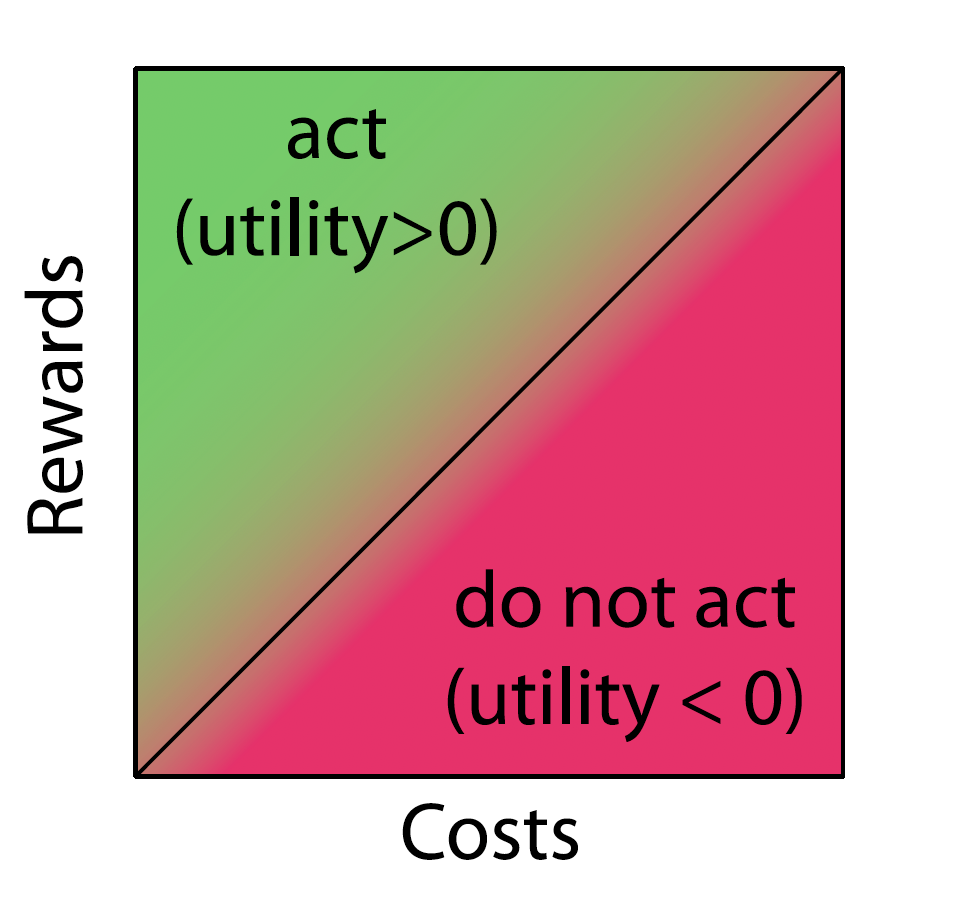
\includegraphics[width=0.8\textwidth]{utility1.png}
\end{center}
\end{column}
\begin{column}{0.5\textwidth}
\pause
\begin{itemize}
    \item Pursue high-cost implies reward was even higher
    \pause
    \item Pursue low-cost does not give info about reward
    \pause
    \item Forego high-cost does not give info about reward
    \pause
    \item Forego low-cost implies reward was even lower
\end{itemize}
\end{column}
\end{columns}
\end{frame}

\begin{frame}
\frametitle{Naive Utility Calculus}
\begin{center}
\Large $U(p, o) = R(o) - C(p)$
\end{center}
\vspace{0.5cm}
\begin{itemize}
    \item $U(p, o)$: utility expected from acting according to plan $p$ to reach outcome $o$
    \item $R(o)$: subjective reward the agent expects from outcome $o$
    \item $C(p)$: subjective cost of executing plan $p$
\end{itemize}
\end{frame}

\begin{frame}
\frametitle{Caveats}
\begin{itemize}
    \item \textbf{Descriptive, not normative:} This is not about how people \textit{should} make decisions (economic utility theory)
    \item \textbf{How we actually operate:} This describes how we \textit{intuitively} make sense of other people's behavior
    \item People don't explicitly compute utilities when they act - this is the cognitive framework we use to understand others
\end{itemize}
\end{frame}

\begin{frame}
\frametitle{Utility and Efficiency}
\begin{center}
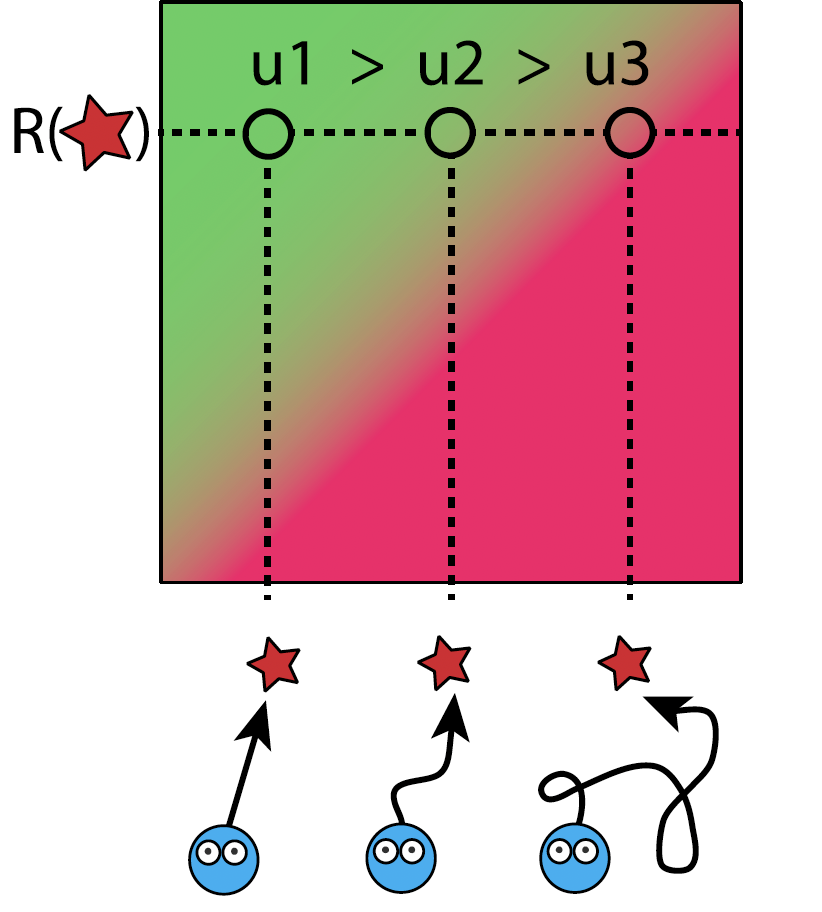
\includegraphics[width=0.3\textwidth]{utility2.png}
\end{center}
\vspace{0.3cm}
\begin{itemize}
    \item More efficient paths are less costly and therefore produce higher utilities
    \item When agents act, they will fulfill their goals as efficiently as possible to maximize utility
\end{itemize}
\end{frame}

\begin{frame}
\frametitle{Graded Preference Inference}
\begin{center}
Does the agent prefer the green or purple star? To what extent? 
\end{center}
\vspace{0.3cm}
\begin{center}
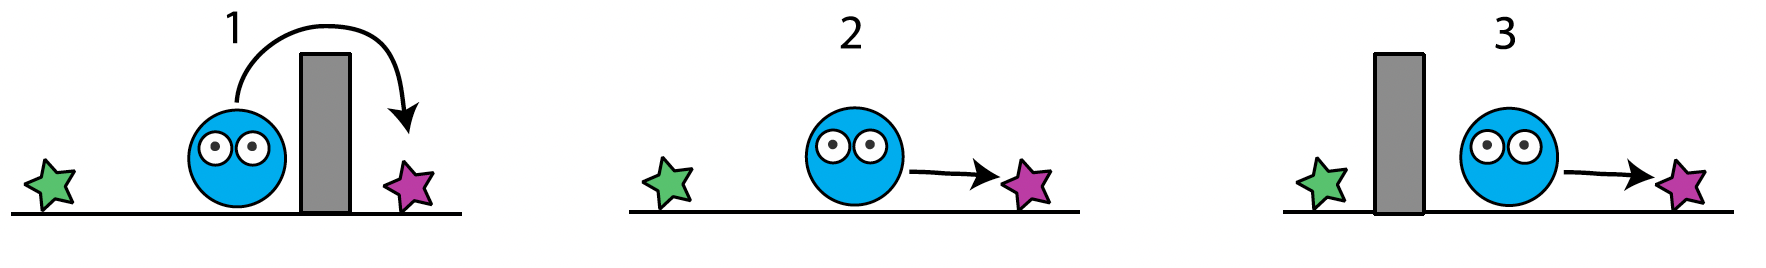
\includegraphics[width=0.7\textwidth]{utility3.png}
\end{center}

\vspace{0.3cm}
\begin{itemize}
    \pause
    \item \textbf{Fig.1: Pursue high-cost}: Agent pays high cost (long detour) to get purple star → strong preference inference
    \pause
    \item \textbf{Fig.2: Pursue low-cost}: Agent pays low cost (short path) to get purple star → weak preference inference
    \pause
    \item \textbf{Fig.3: Forego high-cost}: Agent foregoes high cost (doesn't climb wall) to get green star, chooses purple instead → no preference inference
\end{itemize}
\end{frame}

\begin{frame}
\frametitle{Costs and Rewards Vary Across Agents}
\begin{center}
What do the agent's actions imply about their preferences?
\end{center}
\vspace{0.3cm}
\begin{center}
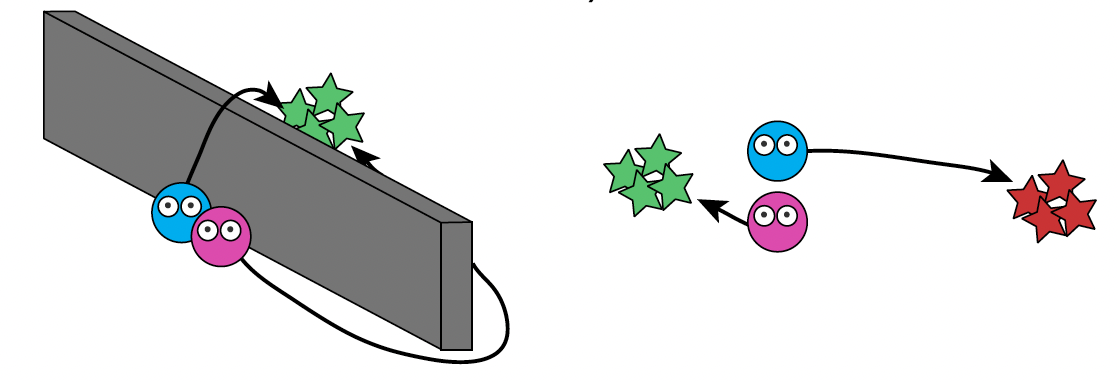
\includegraphics[width=0.7\textwidth]{utility4.png}
\end{center}

\vspace{0.3cm}
\begin{itemize}
    \pause
    \item \textbf{Costs vary}: Blue agent can climb walls easily, pink agent cannot → different action costs
    \pause
    \item \textbf{Rewards vary}: Blue agent prefers red stars, pink agent prefers green stars → different goal values
    \pause
    \item \textbf{Same action, different inference}: Identical behavior can imply different preferences based on agent capabilities and values
\end{itemize}
\end{frame}

\section{Related Work}
\begin{frame}
\frametitle{Feature-Based Approach}
\begin{columns}
\begin{column}{0.5\textwidth}
\begin{center}
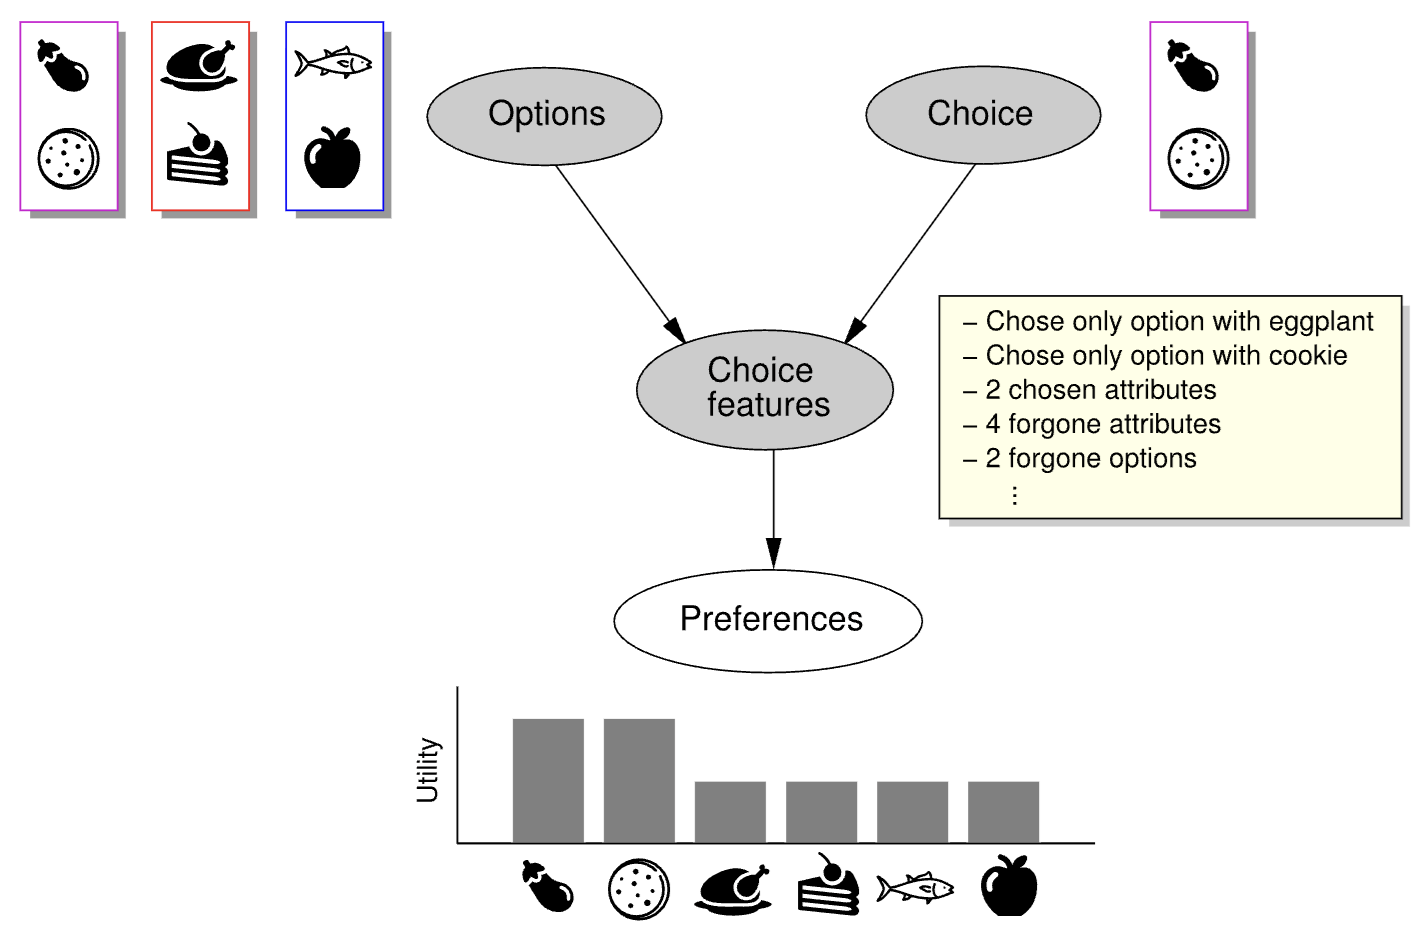
\includegraphics[width=0.95\textwidth]{feature_based.png}
\end{center}
\end{column}
\begin{column}{0.5\textwidth}
\begin{itemize}
    \item \textbf{Method}: Look at simple features of the choice and apply rules
    \item \textbf{Example}: Alice chooses \{eggplant sandwich\} over \{turkey, tuna, ham\}
    \item \textbf{Feature}: "She chose the only option with eggplant"
    \item \textbf{Rule}: "When someone picks the unique option, they probably like that thing"
    \item \textbf{Conclusion}: "Alice likes eggplant"
\end{itemize}
\end{column}
\end{columns}
\end{frame}

\begin{frame}
\frametitle{Inverse Decision-Making Approach}
\begin{columns}
\begin{column}{0.5\textwidth}
\begin{center}
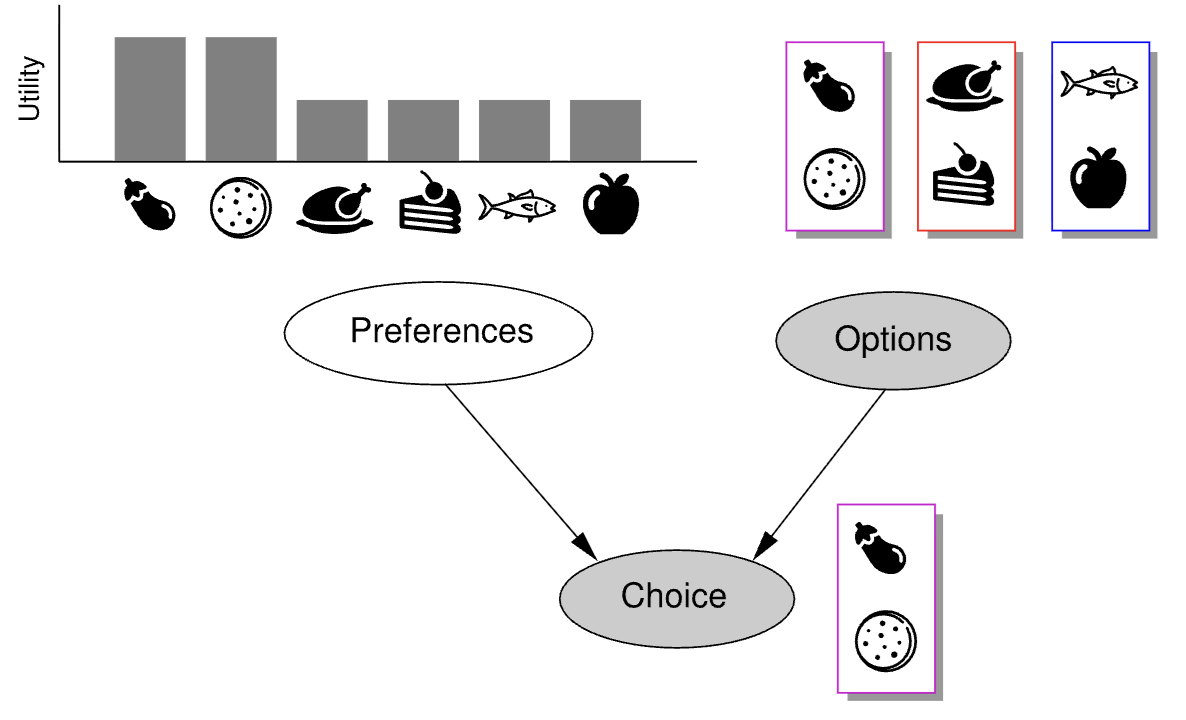
\includegraphics[width=0.95\textwidth]{inverse_decision.png}
\end{center}
\end{column}
\begin{column}{0.5\textwidth}
\begin{itemize}
    \item \textbf{Method}: Use a model of how people actually make decisions, then work backwards
    \item \textbf{Example}: Same choice - Alice chooses \{eggplant sandwich\} over \{turkey, tuna, ham\}
    \item \textbf{Model thinking}: "If Alice really liked eggplant, how likely would she be to make this choice? What if she liked turkey instead? What if she just wanted any sandwich?"
    \item \textbf{Calculation}: Uses math to figure out which preference scenario makes this choice most probable
    \item \textbf{Conclusion}: "Alice probably likes eggplant" (but with precise confidence levels)
\end{itemize}
\end{column}
\end{columns}
\end{frame}

\begin{frame}
\frametitle{NUC vs. Inverse Decision-Making}
\begin{itemize}
    \item \textbf{Similarity}: NUC is similar to inverse decision-making as it works on assumption that agents maximize utilities
    \item \textbf{Key Differences}:
    \begin{itemize}
        \item Uses events with complex spatiotemporal structures and not just isolated discrete choices
        \item Computes both variables costs and rewards, whereas inverse decision-making only infers rewards without costs
    \end{itemize}
\end{itemize}
\end{frame}

\begin{frame}
\frametitle{Inverse Planning}
\begin{columns}
\begin{column}{0.5\textwidth}
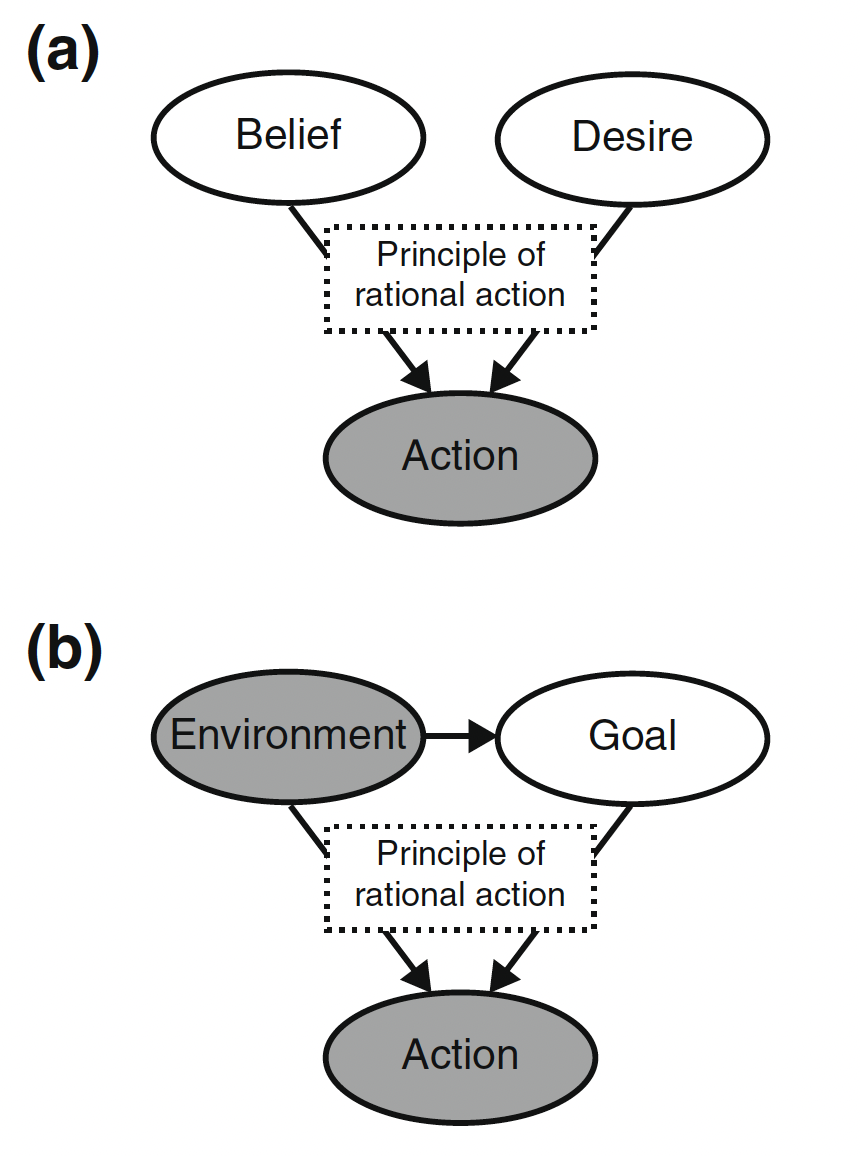
\includegraphics[width=1.0\textwidth]{inverse_planning.png}
\end{column}
\begin{column}{0.5\textwidth}
\textbf{Belief-Desire Psychology ("Forward-thinking")}
\begin{itemize}
    \item Belief + Desire → Action
    \item "Sarah believes store is open + wants coffee → walks to coffee shop"
\end{itemize}

\vspace{0.4cm}
\textbf{Inverse Planning ("Backward-thinking")}
\begin{itemize}
    \item Observe: Environment + Action → Infer: Goal
    \item "See maze layout + this path → agent wants point A"
\end{itemize}
\end{column}
\end{columns}
\end{frame}

\begin{frame}
\frametitle{Goal-Directed Action Understanding}
\begin{columns}
\begin{column}{0.5\textwidth}
\begin{center}
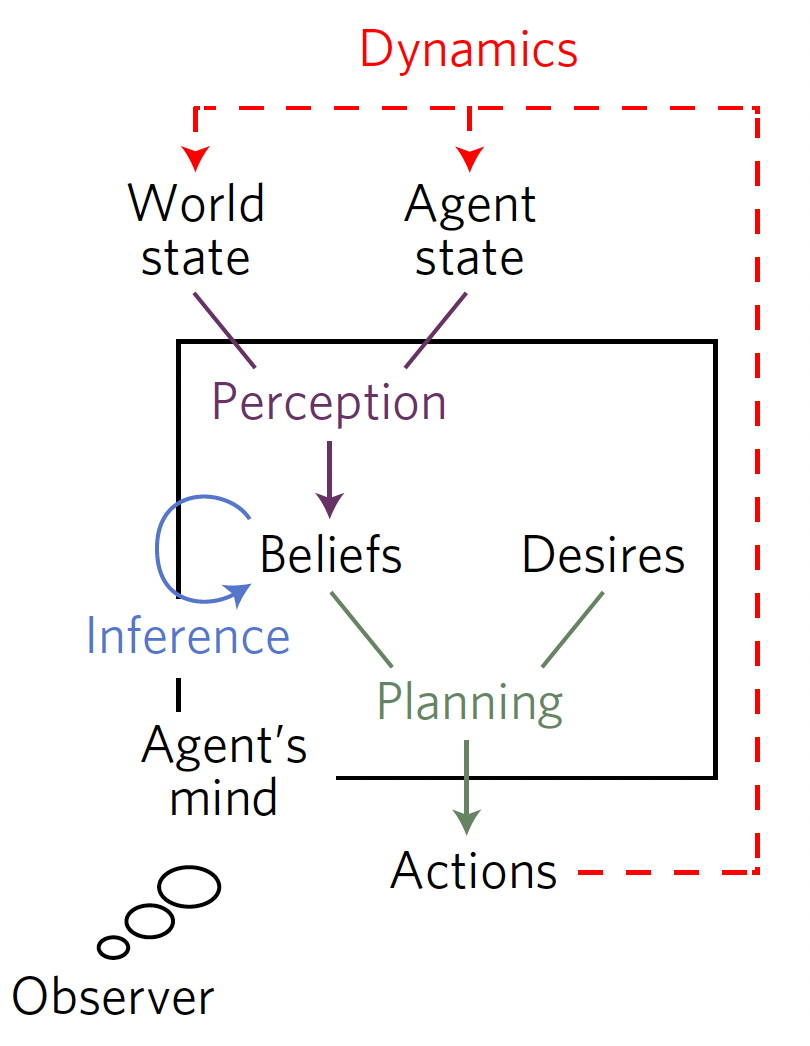
\includegraphics[width=0.95\textwidth]{goal_directed.png}
\end{center}
\end{column}
\begin{column}{0.5\textwidth}
\textbf{Limitations}
\begin{itemize}
    \item Model does not explain multiple causes behind other people's goals
    \item Treats cost as constant, observable and uniform across agents
\end{itemize}
\end{column}
\end{columns}
\end{frame}

\begin{frame}
\frametitle{Research Questions}
\begin{itemize}
    \item \textbf{RQ1}: Can NUC support joint inference of costs and rewards when we know neither, using a coherent generative model?
    \item \textbf{RQ2}: Does NUC drive fine-grained quantitative inferences or only coarse qualitative ones?
    \item \textbf{RQ3}: Is NUC a unified generative model supporting probabilistic inference, or a collection of simple heuristics?
\end{itemize}
\end{frame}

\section{Experiments}

\begin{frame}
\frametitle{Interactive Experiment}
\begin{columns}
\begin{column}{0.4\textwidth}
\begin{center}
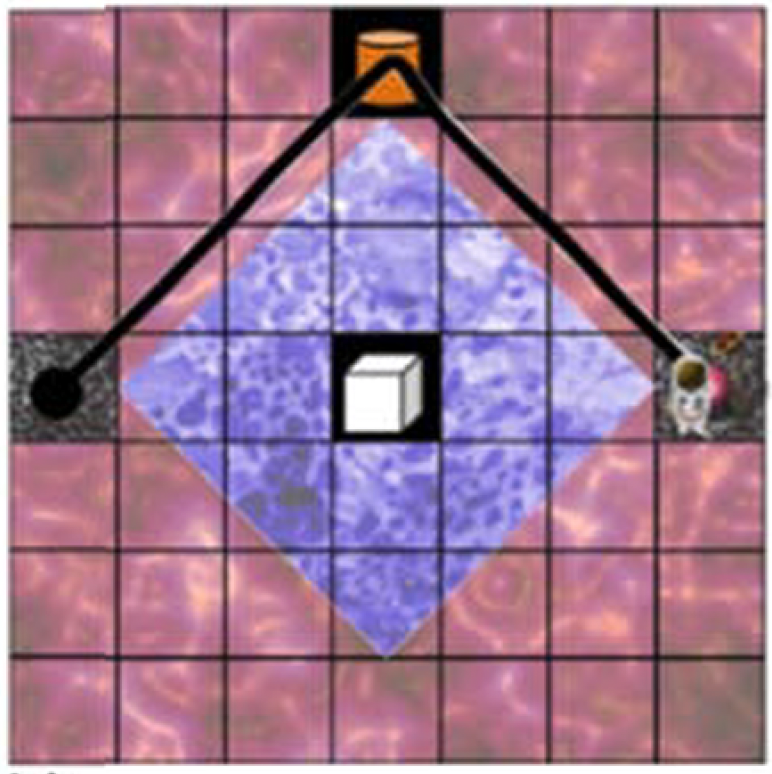
\includegraphics[width=\textwidth]{experiment_1a-1.png}
\end{center}
\end{column}
\begin{column}{0.6\textwidth}
You will watch astronauts land on an alien planet with novel terrains and travel towards their space station. The astronauts can always travel across all types of terrain and can collect up to one care package on their way home.

\vspace{0.5cm}
\textbf{Your Task:} Determine the astronauts'
\begin{itemize}
    \item \textbf{Ability} to travel each kind of terrain (costs)
    \item \textbf{Desire} to collect each care package (rewards)
\end{itemize}
\end{column}
\end{columns}
\end{frame}

\begin{frame}
\frametitle{Quick Check}
\begin{enumerate}
    \item Do astronauts have identical or different abilities?
    \vspace{0.5cm}
    \item Do astronauts have identical or different care package preferences?
    \vspace{0.5cm}
    \item Can astronauts always cross all terrains, even if exhausting?
    \vspace{0.5cm}
    \item How many care packages must/can astronauts collect?
\end{enumerate}
\end{frame}

\begin{frame}
\frametitle{Quick Check}
\begin{enumerate}
    \item Do astronauts have identical or different abilities?
    \begin{itemize}
        \item[\textbf{Answer:}] Different astronauts have different abilities
    \end{itemize}
    \vspace{0.3cm}
    \item Do astronauts have identical or different care package preferences?
    \begin{itemize}
        \item[\textbf{Answer:}] Different astronauts have different preferences
    \end{itemize}
    \vspace{0.3cm}
    \item Can astronauts always cross all terrains, even if exhausting?
    \begin{itemize}
        \item[\textbf{Answer:}] Yes, all astronauts can travel across all terrains
    \end{itemize}
    \vspace{0.3cm}
    \item How many care packages must/can astronauts collect?
    \begin{itemize}
        \item[\textbf{Answer:}] Up to one care package (optional)
    \end{itemize}
\end{enumerate}
\end{frame}

\begin{frame}
\frametitle{Questions to Answer}
\begin{columns}
\begin{column}{0.5\textwidth}
\textbf{For Terrain}\\
"How easy is it to cross this terrain?"

\vspace{0.3cm}
\textbf{Scale:} 0 to 10
\begin{itemize}
    \item \textbf{0} = Extremely easy
    \item \textbf{5} = Average  
    \item \textbf{10} = Extremely exhausting
\end{itemize}
\end{column}
\begin{column}{0.5\textwidth}
\textbf{Care Package}\\
"How much does the astronaut like this container?"

\vspace{0.3cm}
\textbf{Scale:} 0 to 10
\begin{itemize}
    \item \textbf{0} = Not at all
    \item \textbf{5} = Average
    \item \textbf{10} = A lot
\end{itemize}
\end{column}
\end{columns}
\end{frame}

\begin{frame}
    \frametitle{Experiment 1a-1}
    \begin{columns}
    \begin{column}{0.5\textwidth}
    \begin{center}
    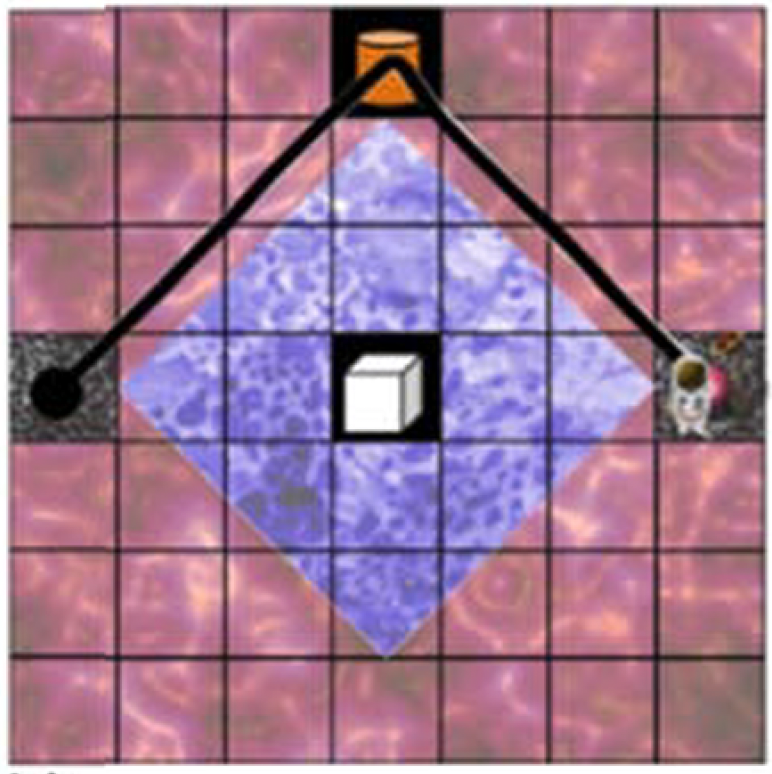
\includegraphics[width=0.9\textwidth]{experiment_1a-1.png}
    \end{center}
    \end{column}
    \begin{column}{0.5\textwidth}
    Based on this astronaut's path, rate on a scale of 0-10:
    
    \vspace{0.2cm}
    \textbf{1. Red terrain} 
\includegraphics[width=0.8cm]{red_terrain.png}\\
    How easy is it to cross?
    \vspace{0.2cm}
    
    \textbf{2. Blue terrain} 
\includegraphics[width=0.8cm]{blue_terrain.png}\\
    How easy is it to cross?
    \vspace{0.2cm}
    
    \textbf{3. White care package} 
\includegraphics[width=0.8cm]{white_carepackage.png}\\
    How much does the astronaut like it?
    \vspace{0.2cm}
    
    \textbf{4. Orange care package} 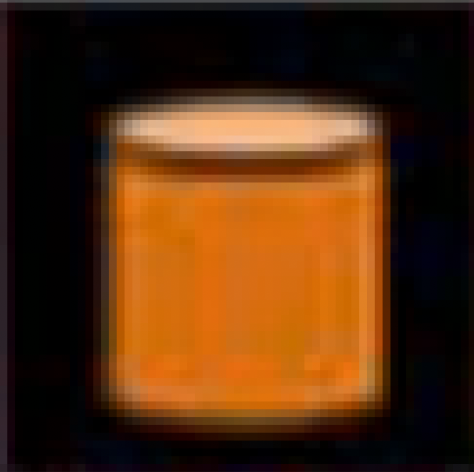
\includegraphics[width=0.8cm]{orange_carepackage.png}\\
    How much does the astronaut like it?
    \end{column}
    \end{columns}
    \end{frame}

\begin{frame}
\frametitle{Experiment 1a-2}
\begin{columns}
\begin{column}{0.5\textwidth}
\begin{center}
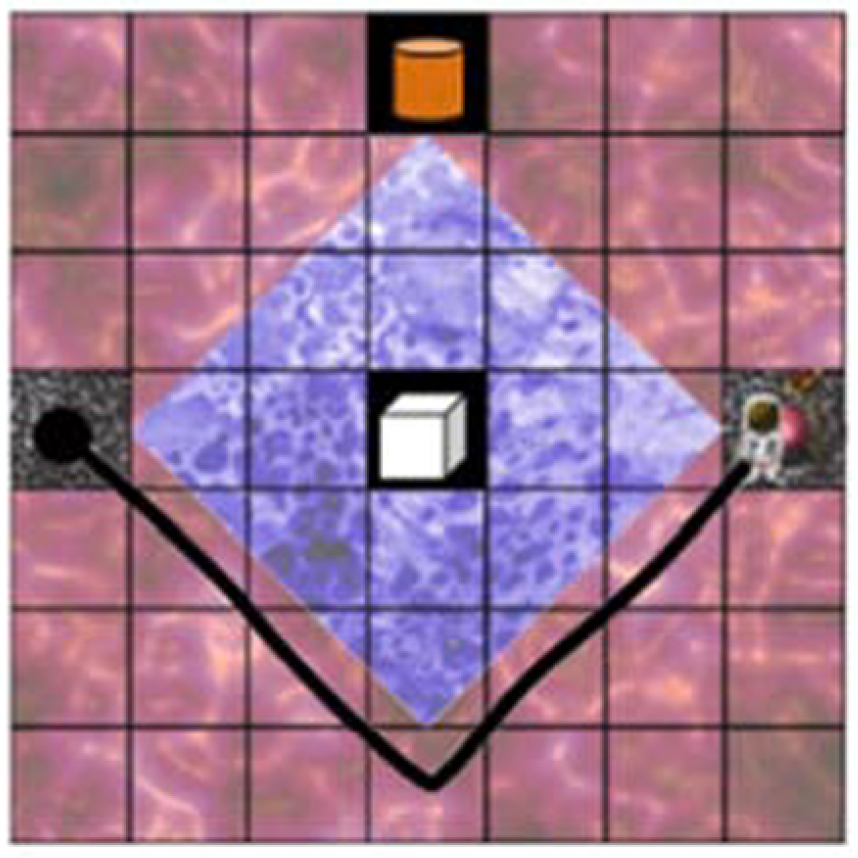
\includegraphics[width=0.9\textwidth]{experiment_1a-2.png}
\end{center}
\end{column}
\begin{column}{0.5\textwidth}
Based on this astronaut's path, rate on a scale of 0-10:

\vspace{0.2cm}
\textbf{1. Red terrain} 
\includegraphics[width=0.8cm]{red_terrain.png}\\
How easy is it to cross?
\vspace{0.2cm}

\textbf{2. Blue terrain} 
\includegraphics[width=0.8cm]{blue_terrain.png}\\
How easy is it to cross?
\vspace{0.2cm}

\textbf{3. White care package} 
\includegraphics[width=0.8cm]{white_carepackage.png}\\
How much does the astronaut like it?
\vspace{0.2cm}

\textbf{4. Orange care package} 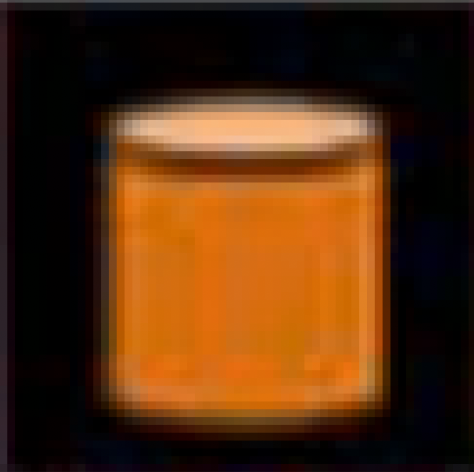
\includegraphics[width=0.8cm]{orange_carepackage.png}\\
How much does the astronaut like it?
\end{column}
\end{columns}
\end{frame}

\begin{frame}
\frametitle{Experiment 1b-1}
\begin{center}
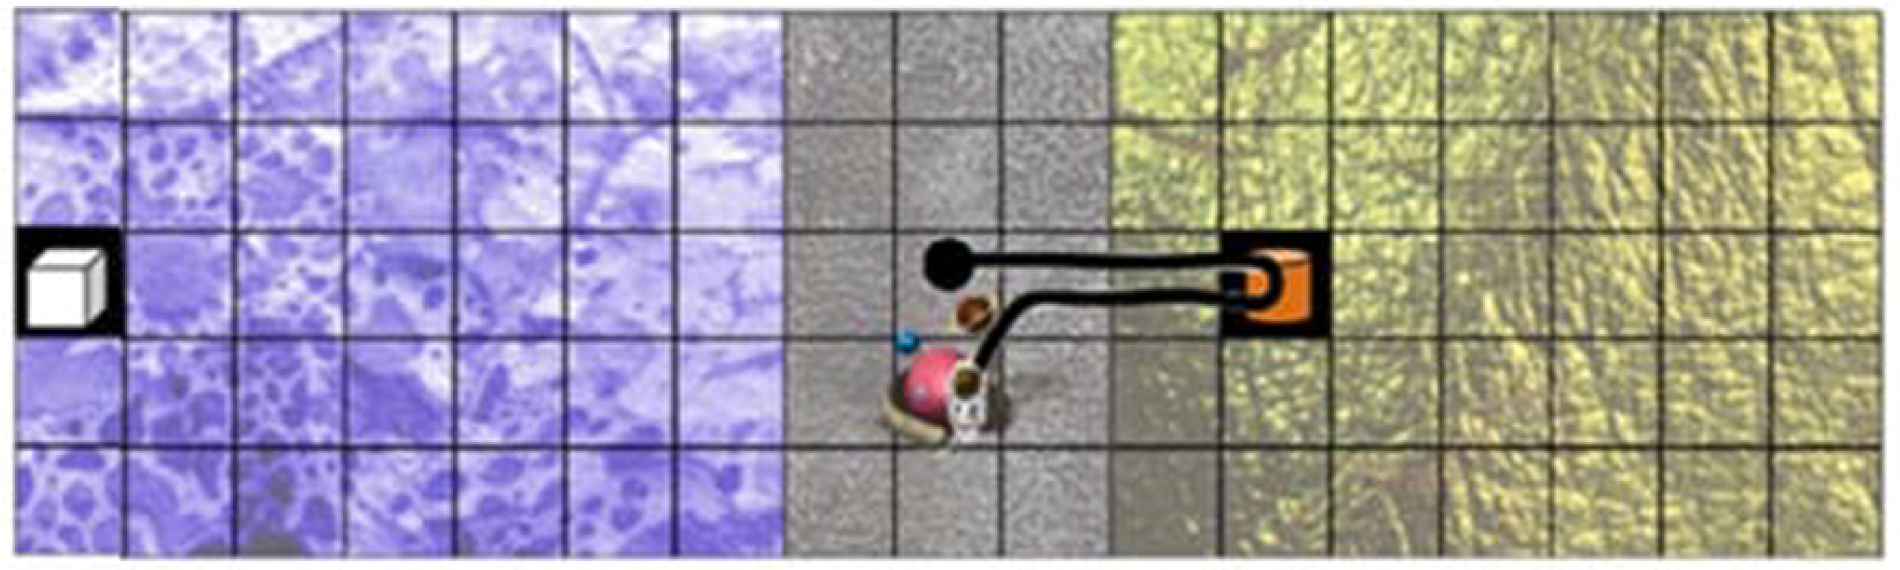
\includegraphics[width=0.8\textwidth]{experiment_1b-1.png}
\end{center}
\vspace{0.3cm}
Based on this astronaut's path, rate on a scale of 0-10:
\begin{columns}
\begin{column}{0.5\textwidth}
\textbf{1. Blue terrain} 
\includegraphics[width=0.8cm]{blue_terrain.png}\\
How easy is it to cross?
\vspace{0.3cm}

\textbf{2. Yellow terrain} 
\includegraphics[width=0.8cm]{yellow_terrain.png}\\
How easy is it to cross?
\end{column}
\begin{column}{0.5\textwidth}
\textbf{3. White care package} 
\includegraphics[width=0.8cm]{white_carepackage.png}\\
How much does the astronaut like it?
\vspace{0.3cm}

\textbf{4. Orange care package} 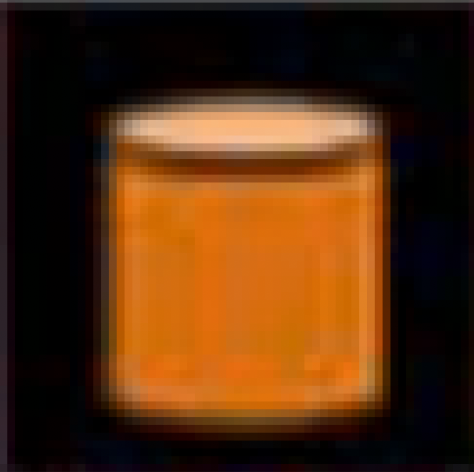
\includegraphics[width=0.8cm]{orange_carepackage.png}\\
How much does the astronaut like it?
\end{column}
\end{columns}
\end{frame}

\begin{frame}
\frametitle{Experiment 1b-2}
\begin{center}
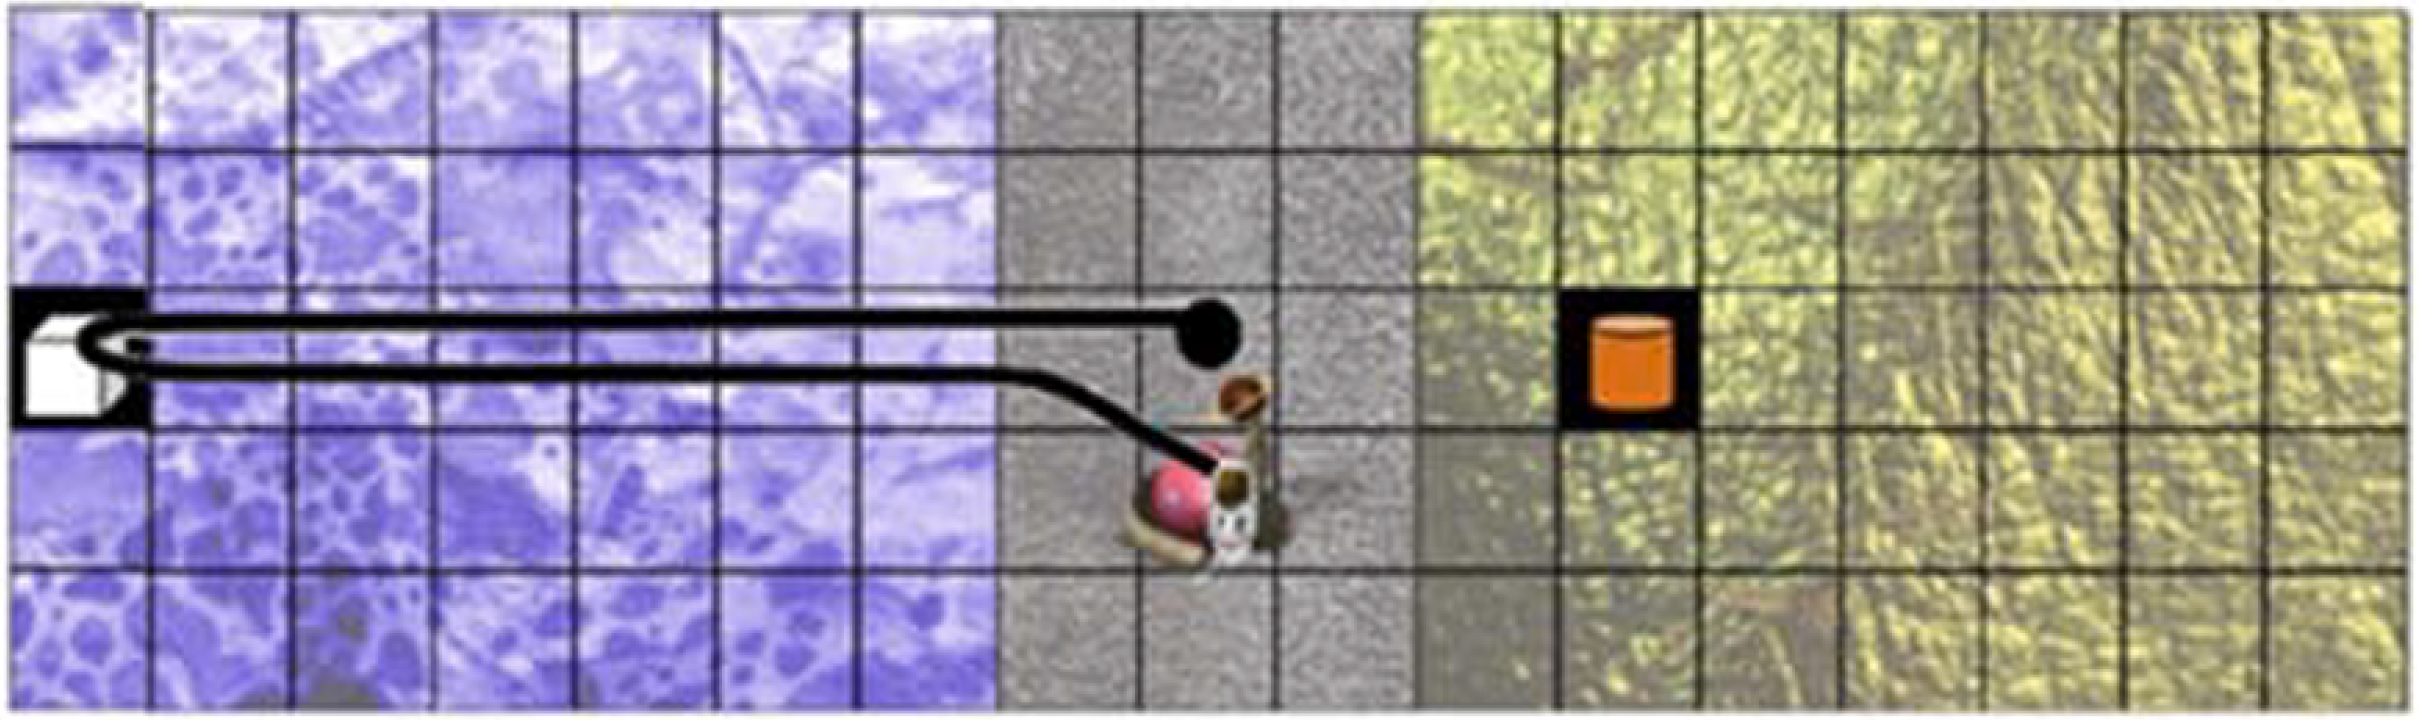
\includegraphics[width=0.8\textwidth]{experiment_1b-2.png}
\end{center}
\vspace{0.3cm}
Based on this astronaut's path, rate on a scale of 0-10:
\begin{columns}
\begin{column}{0.5\textwidth}
\textbf{1. Blue terrain} 
\includegraphics[width=0.8cm]{blue_terrain.png}\\
How easy is it to cross?
\vspace{0.3cm}

\textbf{2. Yellow terrain} 
\includegraphics[width=0.8cm]{yellow_terrain.png}\\
How easy is it to cross?
\end{column}
\begin{column}{0.5\textwidth}
\textbf{3. White care package} 
\includegraphics[width=0.8cm]{white_carepackage.png}\\
How much does the astronaut like it?
\vspace{0.3cm}

\textbf{4. Orange care package} 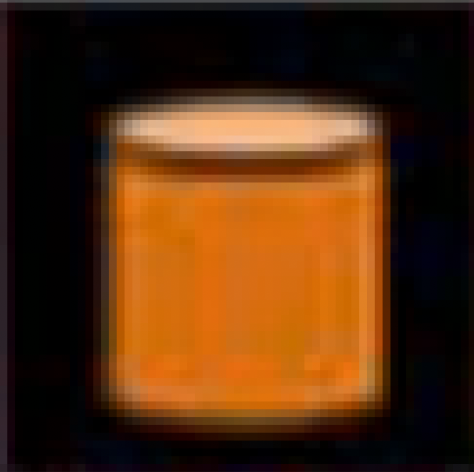
\includegraphics[width=0.8cm]{orange_carepackage.png}\\
How much does the astronaut like it?
\end{column}
\end{columns}
\end{frame}

\begin{frame}
\frametitle{Experiment 1c-1}
\begin{center}
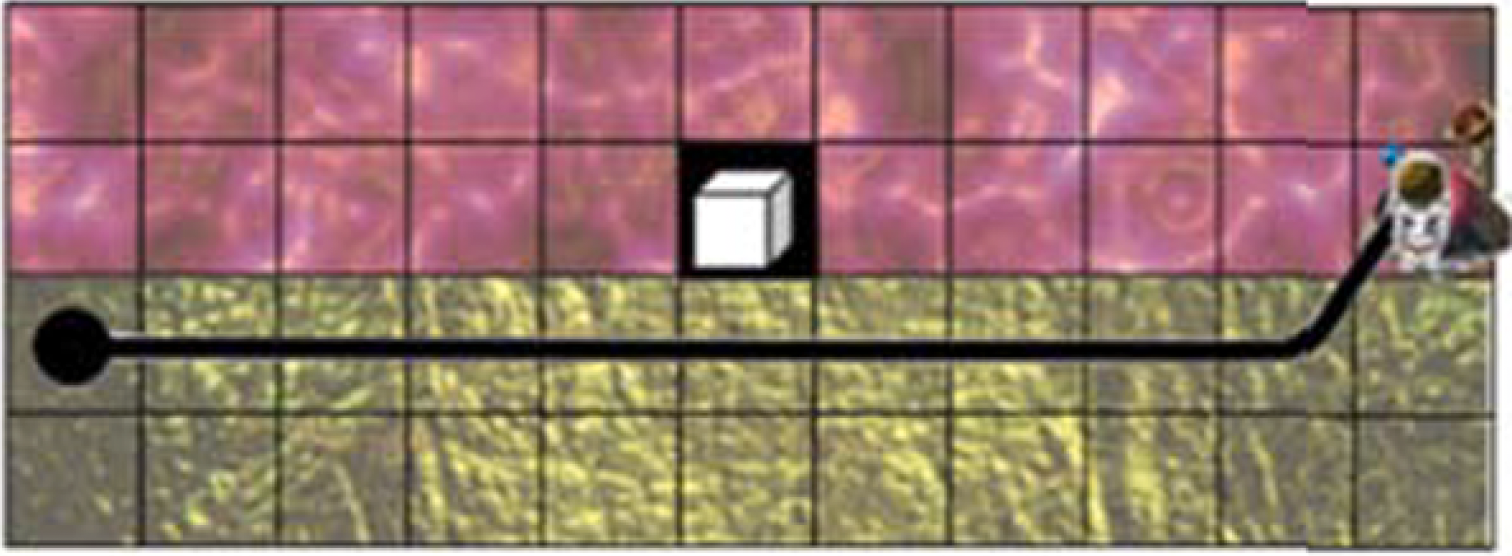
\includegraphics[width=0.8\textwidth]{experiment_1c-1.png}
\end{center}
\vspace{0.3cm}
Based on this astronaut's path, rate on a scale of 0-10:
\begin{columns}
\begin{column}{0.5\textwidth}
\textbf{1. Red terrain} 
\includegraphics[width=0.8cm]{red_terrain.png}\\
How easy is it to cross?
\vspace{0.3cm}

\textbf{2. Yellow terrain} 
\includegraphics[width=0.8cm]{yellow_terrain.png}\\
How easy is it to cross?
\end{column}
\begin{column}{0.5\textwidth}
\textbf{3. White care package} 
\includegraphics[width=0.8cm]{white_carepackage.png}\\
How much does the astronaut like it?
\vspace{0.3cm}
\end{column}
\end{columns}
\end{frame}

\begin{frame}
\frametitle{Experiment 1c-2}
\begin{center}
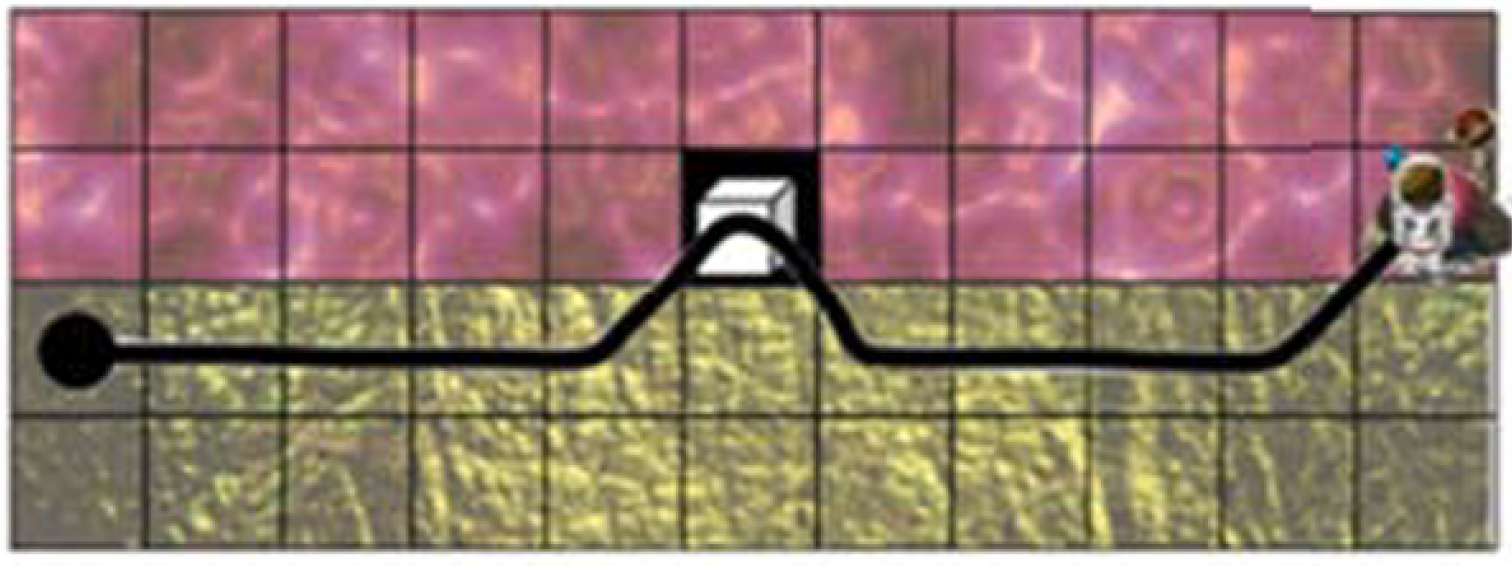
\includegraphics[width=0.8\textwidth]{experiment_1c-2.png}
\end{center}
\vspace{0.3cm}
Based on this astronaut's path, rate on a scale of 0-10:
\begin{columns}
\begin{column}{0.5\textwidth}
\textbf{1. Red terrain} 
\includegraphics[width=0.8cm]{red_terrain.png}\\
How easy is it to cross?
\vspace{0.3cm}

\textbf{2. Yellow terrain} 
\includegraphics[width=0.8cm]{yellow_terrain.png}\\
How easy is it to cross?
\end{column}
\begin{column}{0.5\textwidth}
\textbf{3. White care package} 
\includegraphics[width=0.8cm]{white_carepackage.png}\\
How much does the astronaut like it?
\vspace{0.3cm}
\end{column}
\end{columns}
\end{frame}

\begin{frame}
\frametitle{Experiment Types}
Participants watched agents navigate worlds with different terrains and care packages to infer cost and reward functions. Three different geometries were used:

\vspace{0.3cm}
\begin{itemize}
    \item \textbf{Experiment 1a}: Detours could be explained by either terrain costs or reward differences
    
    \item \textbf{Experiment 1b}: Forced terrain crossings vs. optional detours to collect care packages
    
    \item \textbf{Experiment 1c}: Minimal physical detours that still reveal agent preferences
\end{itemize}

\vspace{0.3cm}
Responses evaluated against Naïve Utility Calculus model and two alternative models.
\end{frame}

\begin{frame}
\frametitle{Experiment 2}
\begin{columns}
\begin{column}{0.5\textwidth}
\begin{center}
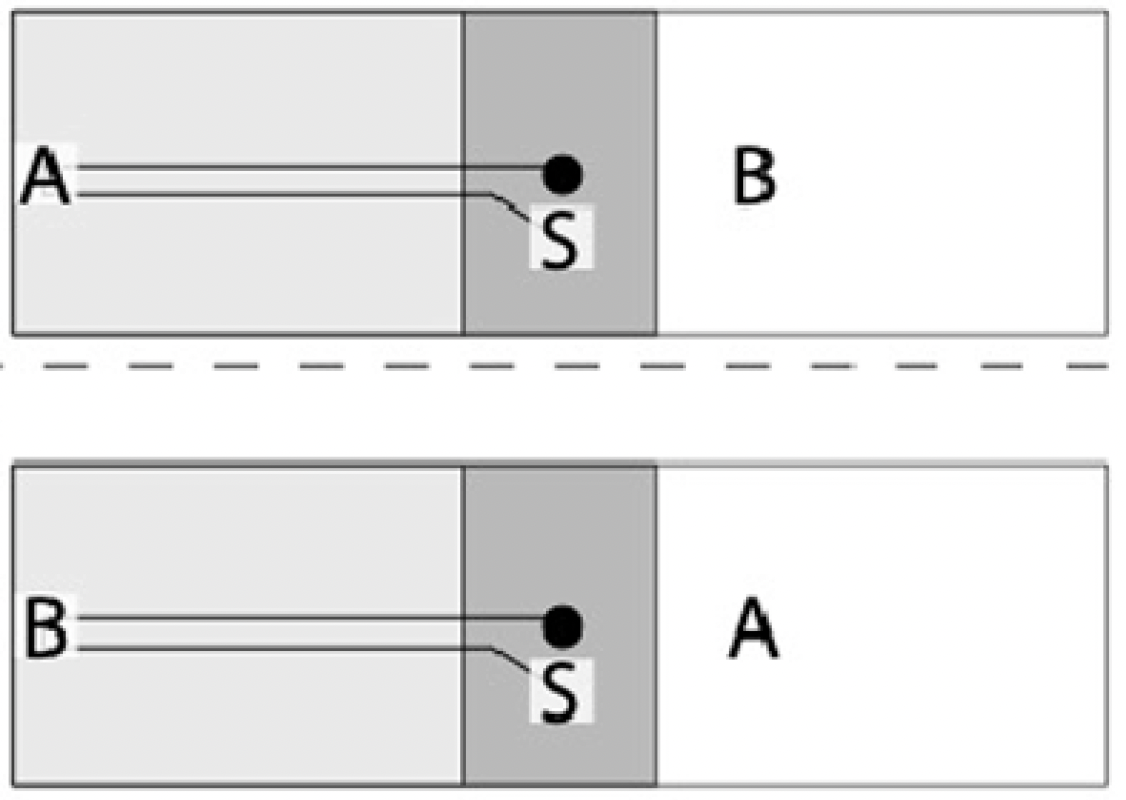
\includegraphics[width=0.9\textwidth]{experiment2-1.png}
\end{center}
\end{column}
\begin{column}{0.5\textwidth}
Based on this astronaut's path across both maps, rate on a scale of 0-10:

\vspace{0.2cm}
\textbf{1. White terrain}\\
How easy is it to cross?
\vspace{0.2cm}

\textbf{2. Gray terrain}\\
How easy is it to cross?
\vspace{0.2cm}

\textbf{3. Reward A}\\
How much does the astronaut like it?
\vspace{0.2cm}

\textbf{4. Reward B}\\
How much does the astronaut like it?
\end{column}
\end{columns}
\end{frame}

\begin{frame}
\frametitle{Why Experiment 2?}
Unlike Experiment 1's single events, real-world observations involve multiple actions across different contexts that let us revise beliefs about agents' costs and rewards.

\vspace{0.3cm}
Experiment 2 tests inference from multiple action events with two purposes:

\vspace{0.3cm}
\begin{itemize}
    \item Test if inferences over repeated events follow the full Naïve Utility Calculus model
    \item Test if a simpler single-event model (using first or most recent observation) explains inferences equally well
\end{itemize}
\end{frame}

\begin{frame}
\frametitle{Processing Human Data to "Ground Truth"}
\textbf{Step 1: Raw Data Collection}
\begin{itemize}
    \item Participants rated on 0-10 scales: terrain difficulty (0=easy, 10=exhausting) and care package preference (0=not at all, 10=a lot)
\end{itemize}

\vspace{0.2cm}
\textbf{Step 2: Z-Scoring Within Each Participant}
\begin{itemize}
    \item Remove individual scale usage differences by standardizing each participant's responses: z = (raw\_response - $\mu$\_participant) / $\sigma$\_participant
\end{itemize}

\vspace{0.2cm}
\textbf{Step 3: Separate by Question Type}
\begin{itemize}
    \item Split z-scored responses into cost judgments and reward judgments
\end{itemize}

\vspace{0.2cm}
\textbf{Step 4: Average Across Participants}
\begin{itemize}
    \item For each trial, average z-scores across all participants to create the "ground truth" score
\end{itemize}
\end{frame}

\begin{frame}
\frametitle{Discussion Questions}
\begin{enumerate}
    \item What limitations are there to using humans as the "ground truth" here?
    \item Is it fair to isolate actions that result in costs and rewards? e.g. What changes if terrains have rewards or care packages have costs?
\end{enumerate}
\end{frame}

% \begin{frame}
% \frametitle{Experiment 5: Joint Cost-Reward Inference}
% \begin{itemize}
%     \item \textbf{Question}: Can people jointly infer costs and rewards from agent behavior?
%     \item \textbf{Design}: Agents with unknown capabilities and unknown goal preferences
%     \item \textbf{Manipulation}: Multiple trials revealing different cost-reward tradeoffs
%     \item \textbf{Results}:
%     \begin{itemize}
%         \item People successfully inferred both costs and rewards simultaneously
%         \item Judgments consistent with Bayesian model predictions
%         \item Performance improved with more observations
%     \end{itemize}
%     \item \textbf{Conclusion}: NUC supports complex joint inference in realistic scenarios
% \end{itemize}
% \end{frame}

\section{Naive Utility Calculus}

\begin{frame}
\frametitle{Key Question}
\begin{center}
\Large How do we design an algorithm that can give us the cost and reward function for each terrain and care package?
\end{center}

\vspace{0.5cm}
\textbf{The intuitive solution involves:}

\vspace{0.3cm}
\begin{enumerate}
    \item \textbf{Generation (Forward):} Given cost and reward → predict actions
    \item \textbf{Inference (Backward):} Given the actions → Infer the costs / rewards
\end{enumerate}
\end{frame}

\begin{frame}
\frametitle{Generative model}
\begin{center}
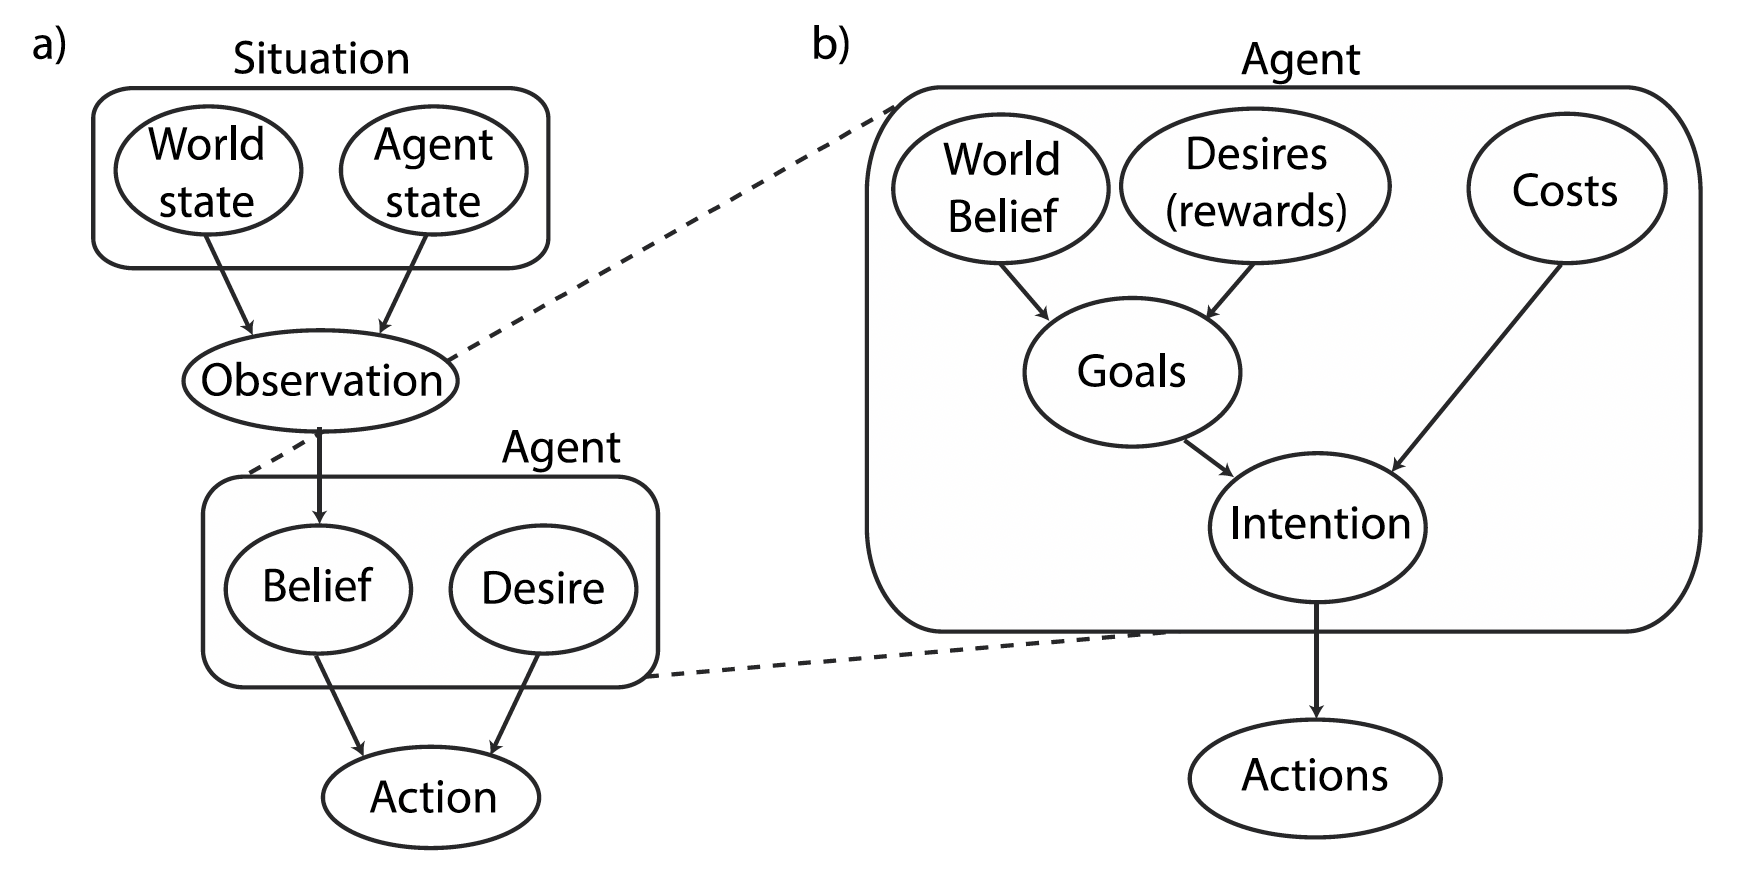
\includegraphics[width=0.6\textwidth]{generative_model.png}
\end{center}

\vspace{0.5cm}
\begin{itemize}
    \pause
    \item \textbf{Desires} = Reward Function
    \pause
    \item \textbf{Goals} = States of the world that the agent believes yield rewards
    \pause
    \item \textbf{Intentions} = Ordered sequences of goals intended to maximize utilities
    \pause
    \item \textbf{Actions} = mappings from states to action which when executed sequentially fulfill each goal in the intention
\end{itemize}
\end{frame}

\begin{frame}
\frametitle{Generative Model}
\begin{center}
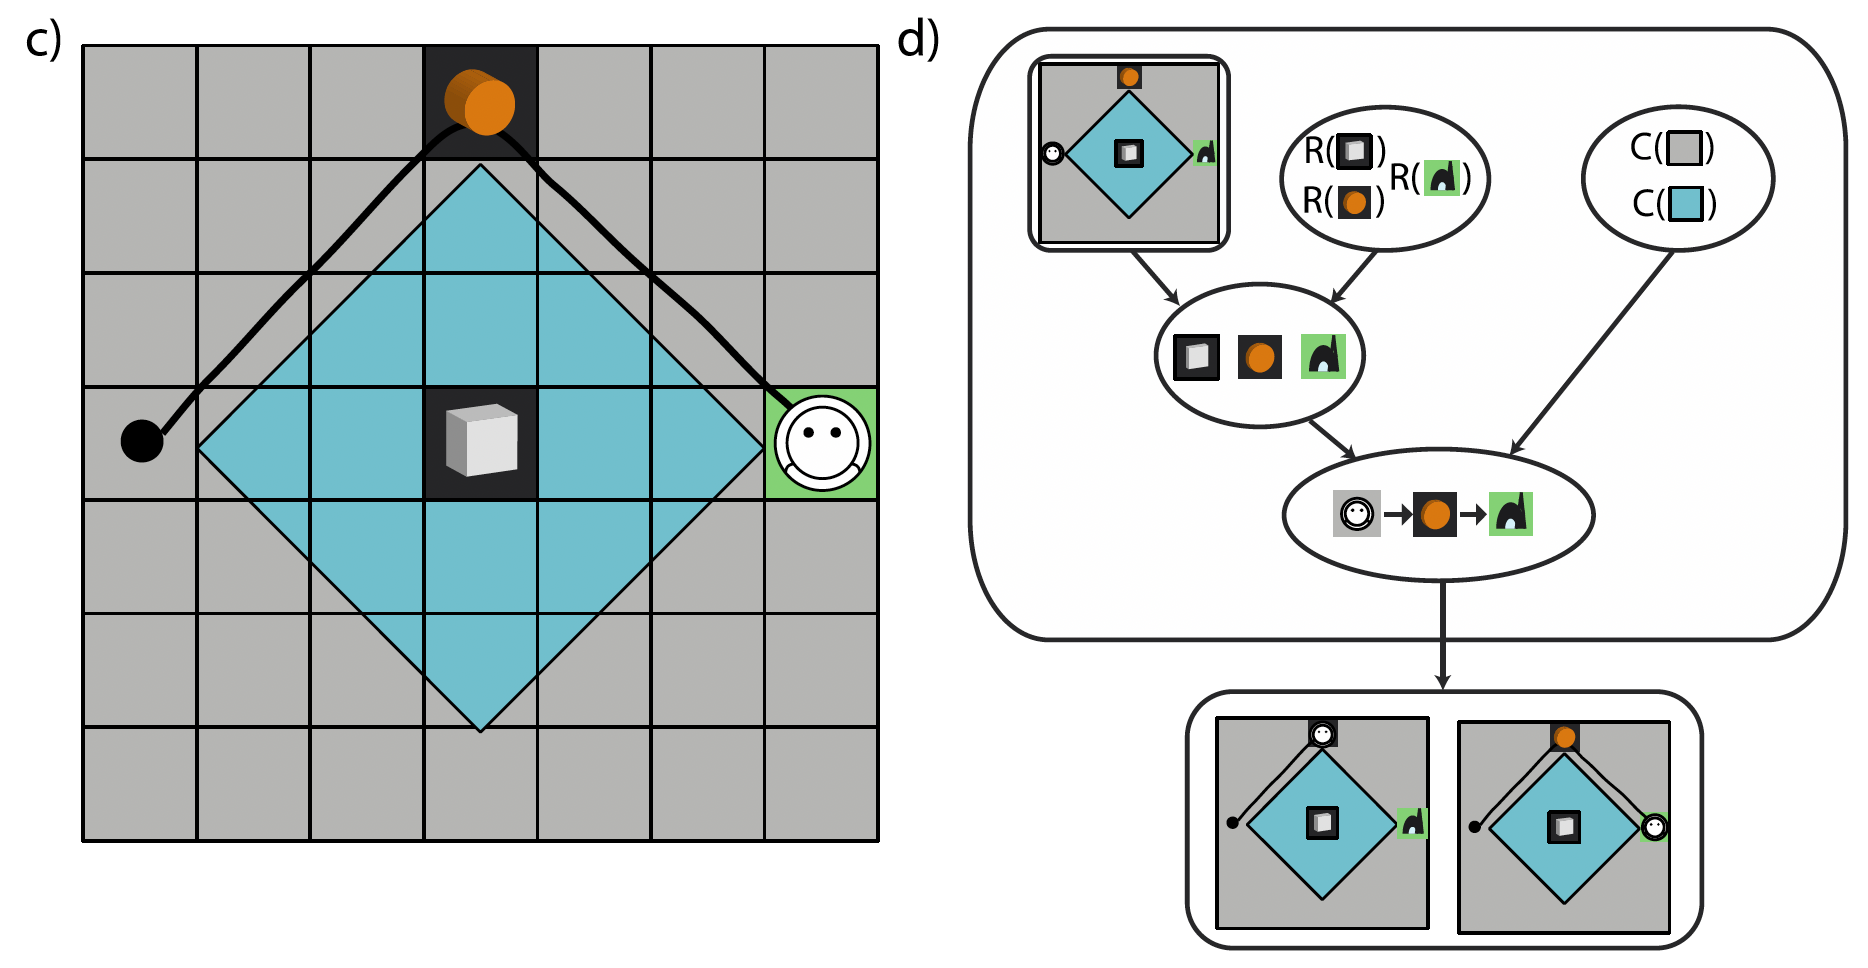
\includegraphics[width=0.6\textwidth]{generative_model2.png}
\end{center}

\vspace{0.3cm}
\begin{itemize}
    \pause
    \item \textbf{Beliefs + Rewards} → Candidate goals
    \pause
    \item \textbf{Goals + Action costs} → Specific intentions to act
    \pause
    \begin{itemize}
        \item Constraint: space station must be final goal
        \item Results in 5 possible intentions: direct path, single package routes, dual package routes
    \end{itemize}
\end{itemize}
\end{frame}

\begin{frame}
\frametitle{Markov Decision Processes (MDPs)}
\begin{columns}
\begin{column}{0.4\textwidth}
\begin{center}
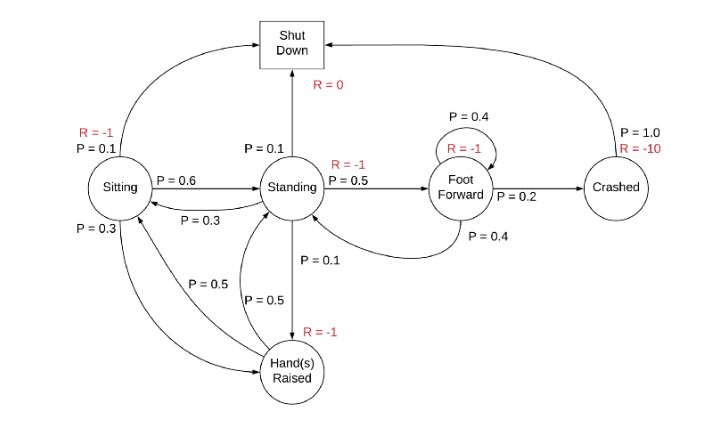
\includegraphics[width=0.9\textwidth]{mdp.png}
\end{center}
\end{column}
\begin{column}{0.6\textwidth}
\textbf{Formal definition:} 4-tuple $(S, A, P_a, R_a)$
\begin{itemize}
    \item \textbf{States} (S): Agent positions
    \item \textbf{Actions} (A): 8 movement directions  
    \item \textbf{Transition probabilities} ($P_a$): Not important here (deterministic)
    \item \textbf{Rewards} ($R_a$): Only at goals
\end{itemize}

\vspace{0.3cm}
\textbf{In NUC context:}
\begin{itemize}
    \item Actions are deterministic
    \item Costs vary by terrain type
    \item Each goal has its own MDP
\end{itemize}
\end{column}
\end{columns}

\vspace{0.3cm}
\textbf{Purpose:} Compute optimal policies to reach goals efficiently, which observers use to infer agent preferences from observed behavior.
\end{frame}

\begin{frame}
\frametitle{Intentions to Action Policies}
\textbf{Intentions:} Ordered sequence of goals (target positions)

\vspace{0.2cm}
\textbf{Utility:} $U = \text{Rewards} - \text{Costs}$

\vspace{0.2cm}
\textbf{Implementation via MDPs:}
\begin{itemize}
    \item Each goal gets its own MDP with single reward at target location
    \item Cost functions: $C: A \times S \rightarrow \mathbb{R}$ (terrain-dependent)
    \item Diagonal moves cost $\sqrt{2} \times$ cardinal moves
\end{itemize}

\vspace{0.2cm}
\textbf{Policy computation (Value Iteration):}
$$V(s) = \max_a \sum_{s'} P^a_{s,s'} V(s') + R(a,s) - C(a,s)$$

\vspace{0.2cm}
\textbf{Softmax policy:} $p(a|s) \propto \exp(\alpha \sum_{s'} P^a_{s,s'} V(s'))$ where $\alpha = 0.1$
\end{frame}


\section{Discussion}
\begin{frame}
\frametitle{Discussion}
\begin{itemize}
    \item \textbf{Key Findings}: People use Naive Utility Calculus for preference inference
    \begin{itemize}
        \item Make graded inferences based on action efficiency
        \item Consider individual differences in costs and rewards
        \item Perform complex joint inference of multiple variables
    \end{itemize}
    \item \textbf{Theoretical Contribution}: NUC as a unified computational framework
    \begin{itemize}
        \item Goes beyond simple heuristics
        \item Supports probabilistic inference mechanisms
        \item Handles spatiotemporal action sequences
    \end{itemize}
    \item \textbf{Future Directions}: 
    \begin{itemize}
        \item Real-world applications beyond gridworlds
        \item Neural mechanisms underlying utility-based reasoning
        \item Cross-cultural and developmental studies
    \end{itemize}
\end{itemize}
\end{frame}

\end{document}